
\section{tikz}


\begin{frame}
	\frametitle{标题}	
	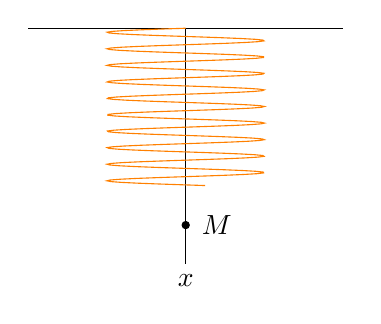
\begin{tikzpicture}
			\draw  (-2,0) -- (2,0) node[below] {};
			\draw  (0,0) -- (0,-3) node[below] {$x$};	
			\draw [orange, domain=0:-2, samples=200] plot({sin(\x r *30},\x);
			\draw [fill, black, circle] (0,-2.5) circle(0.3ex) node[right] {$M$};
  \end{tikzpicture} 
	
\end{frame}

%%%%%%%%%%%%%%%%%%%%%%%%%%%%%%%%%%%%%%%%%%%%%%%%%

\section{区块环境}

\begin{frame}
\frametitle{1.block}
	\begin{block}{勾X定理:}
		直角三角形的斜边的平方等于两直角边的平方和。
		可以用符号语言表述为:设直角三角形ABC,其中$\angle C=90^\circ $则有
		\begin{equation}
			AB^2=BC^2+AC^2 \int
		\end{equation}
	\end{block}
	\begin{block}{Remark}
		Sample text
	\end{block}
\end{frame}

\begin{frame}
    \frametitle{2.alertblock}
	\begin{alertblock}{Important theorem}
		Sample text in red box
	\end{alertblock}
\end{frame}

\begin{frame}
    \frametitle{3.exampleblock}
	\begin{exampleblock} {Exampleblock}
		Sample text in green box. The title of the block is ``Examples".
	\end{exampleblock}
    \begin{exampleblock} {例1:}
		Sample text in green box. The title of the block is ``Examples".
	\end{exampleblock}
\end{frame}

\begin{frame}
    \frametitle{4.examples}
	\begin{examples}
		Sample text in green box. The title of the block is ``Examples".
	\end{examples}
\end{frame}

\begin{frame}
    \frametitle{5.proof}
    \begin{proof}{}
      This is a proof
    \end{proof}
\end{frame}

\begin{frame}
    \frametitle{6.tcolorbox}
    \begin{tcolorbox1}{tcolorbox1}
      This is tcolorbox1 that I defined
    \end{tcolorbox1}
    \begin{tcolorbox1}[2]{定理}
      This is tcolorbox1
    \end{tcolorbox1}
    \begin{tcolorbox2}{tcolorbox2}
      This is tcolorbox2 that I defined
    \end{tcolorbox2}
    \begin{tcolorbox}[title=tcolorbox]
      This is tcolorbox
    \end{tcolorbox}
\end{frame}

\begin{frame}
    \frametitle{7.tcbitemize}

    \tcbset{colback=white,arc=0mm,width=(\linewidth-4pt)/4,
    equal height group=AT,before=,after=\hfill,fonttitle=\bfseries}
    
    \noindent
    \foreach \n in {xxx,ggg,AAA,\"Agypten}
    {\begin{tcolorbox}[title=\n,colframe=red!75!black]
      Some content.\end{tcolorbox}}
    
    \noindent
    \foreach \n in {xxx,ggg,AAA,\"Agypten}
    {\begin{tcolorbox}[adjusted title=\n,colframe=blue!75!black]
    Some content.\end{tcolorbox}}
    
    \begin{tcbitemize}[raster columns=3,raster equal height,
              colframe=red!75!black,colback=red!5!white,fonttitle=\bfseries]
    \tcbitem[squeezed title={Short title}]
    First box
    \tcbitem[squeezed title={This is a very very long title}]
    Second box
    \tcbitem[squeezed title={This title is clearly to long for this application}] Third box
    \end{tcbitemize}
    
    \begin{tcbitemize}[raster columns=3,raster equal height,
              colframe=blue!75!black,colback=red!5!white,fonttitle=\bfseries]
    \tcbitem[squeezed title*={Short title}]
    First box
    \tcbitem[squeezed title*={This is a very very long title}]
    Second box
    \tcbitem[squeezed title*={This title is clearly to long for this application}] Third box
    \end{tcbitemize}
  \end{frame}


%%%%%%%%%%%%%%%%%%%%%%%%%%%%%%%%%%%%%%%%%%%%%%%%%
\begin{frame}
	\begin{center}
		\huge Thanks for your attention! \\ Q \& A
	\end{center}
\end{frame}

%%%%%%%%%%%%%%%%%%%%%%%%%%%%%%%%%%%%%%%%%%%%%%%%%

